\documentclass[10pt, xcolor=x11names, compress]{beamer}
%\documentclass[10pt, xcolor=x11names, compress, handout]{beamer}

\usetheme{progressbar}
%\usecolortheme[named=Purple4]{structure}
\progressbaroptions{headline=sections,titlepage=normal,frametitle=normal}

\setbeamertemplate{navigation symbols}{}

\usepackage{iwona} 

\usepackage{alltt}
\usepackage{amsmath,amsfonts, amssymb, amscd}
\usepackage{hyperref}
\usepackage{setspace}
\usepackage{wasysym}
\usepackage{ulem}

\usepackage{calc}
\usepackage[overlay,absolute]{textpos}
\TPGrid[5mm,5mm]{20}{20}


\renewcommand{\Re}{\operatorname{Re}}
\renewcommand{\Im}{\operatorname{Im}}
\newcommand{\debye}{\operatorname{debye}}

\newcommand{\chik}{$\chi(k)$}
\newcommand{\chir}{$|\tilde{\chi}(R)|$}


\newcommand{\file}[1]{{\color{Firebrick4}\texttt{`#1'}}}
\newcommand{\multiple}{{\color{Orange3}\textsl{multiple}}}


\newcommand{\atoms}  {{\color{DarkOrchid4}\textsc{atoms}}}
\newcommand{\feff}   {{\color{DarkOrchid4}\textsc{feff}}}
\newcommand{\ifeffit}{{\color{DarkOrchid4}\textsc{ifeffit}}}
\newcommand{\athena} {{\color{DarkOrchid4}\textsc{athena}}}
\newcommand{\artemis}{{\color{DarkOrchid4}\textsc{artemis}}}

\renewenvironment<>{center}
{\begin{actionenv}#1\begin{originalcenter}}
{\end{originalcenter}\end{actionenv}}

\mode<presentation>
%\mode<beamer>

\title{Your Second EXAFS Lecture}%
\subtitle{In which we explore the ins and outs of absorption
  spectroscopy, learn of some the ways to interpret our data, and
  prepare for the rest of this XAFS course}

\author{Bruce Ravel}
\institute[NIST]{Synchrotron Methods Group, Materials Measurement Science Division\\%
  Materials Measurement Laboratory\\%
  National Institute of Standards and Technology\\%
  \&\\%
  Local Contact, Beamline X23A2\\%
  National Synchrotron Light Source\\~}



\date[Diamond2011]{EXAFS Data Analysis workshop 2011\\
  Diamond Light Source\\November 14--17, 2011}

\begin{document}
\begin{frame}
  \titlepage
\end{frame}

\begin{frame}
  \frametitle{Copyright}
  \tiny

  This document is copyright \copyright 2007-2010 Bruce Ravel.

  \begin{center}
    
\includegraphics[width=1.0cm]{images/somerights20}
  \end{center}

  This work is licensed under the Creative Commons
  Attribution-ShareAlike License.  To view a copy of this license,
  visit \href{http://creativecommons.org/licenses/by-sa/3.0/}
  {\color{Purple4}\texttt{http://creativecommons.org/licenses/by-sa/3.0/}}
  or send a letter to Creative Commons, 559 Nathan Abbott Way,
  Stanford, California 94305, USA.

  \begin{description}
  \item[You are free:] %
    \begin{itemize}
    \item \textbf{to Share} --- to copy, distribute, and transmit the work
    \item \textbf{to Remix} --- to adapt the work
    \end{itemize}
  \item[Under the following conditions:] %
    \begin{itemize}
    \item Attribution. You must attribute the work in the manner
      specified by the author or licensor (but not in any way that
      suggests that they endorse you or your use of the work).
    \item Share Alike. If you alter, transform, or build upon this
      work, you may distribute the resulting work only under the same,
      similar or a compatible license.
    \item Any of these conditions can be waived if you get permission
      from the author.
    \end{itemize}
  \end{description}
  \begin{itemize}
  \item For any reuse or distribution, you must make clear to others
    the license terms of this work. The best way to do this is with a
    link to the URL for this document.
  \item Any of the above conditions can be waived if you get
    permission from the copyright holder.
  \item Nothing in this license impairs or restricts the author's
    moral rights.
  \end{itemize}

  Your fair dealing and other rights are in no way affected by the
  above.  This is a human-readable summary of the Legal Code (the full
  license).


\end{frame}

%%% Local Variables:
%%% mode: latex
%%% TeX-master: "pimst2"
%%% End:


\begin{frame}
  \frametitle{Abstract}
  This lecture is the introductory lecture to a short course on the
  technique of X-ray Absorption Spectroscopy and the anaylsis of XAS
  data.  This is not a ground-level introduction for the complete
  beginner.  We will not derive the EXAFS equation nor explore the
  fundamental physics of the interaction between the photon and the
  absorbing atom.  I assume that you have already been to the
  synchrotron and measured some XAS data.

  \medskip

  The lecture will set the stage for what is to come in this short
  course.  We will motivate the importance of studying XAS in depth,
  even for those who will never make the practice of XAS their primary
  occupation.  We will see an overview of many of the ways to
  interpret and analyze your XAS data.  Finally, we look ahead to the
  end of the course to consider how good experimental practice and
  attention to statistics benefit every XAS practitioner.
\end{frame}

\begin{frame}
  \frametitle{Acknowledgements}
  \begin{columns}[T]
    \begin{column}{0.9\linewidth}
      \begin{itemize}
        \footnotesize
      \item Matt Newville, the author of \textsc{ifeffit}, without
        which \textsc{athena} and \textsc{artemis} would not exist.
      \item Shelly Kelly and Scott Calvin, old friends, relentless
        finders of software bugs, and long-time co-conspirators in
        this XAS eductaion gig
      \item My teachers, Ed Stern and John Rehr, who have done so much
        for the XAS community and who instilled in me a love of the
        discipline of XAS
      \item My most wonderful boss, Dan Fischer, for letting me duck
        out of work to do things like this
      \item The folks who make the great software I use to write my codes:
        \href{http://www.perl.org}{\color{Blue4}Perl},
        \href{http://wxperl.sourceforge.net/}{\color{Blue4}wxPerl},
        \href{http://www.gnu.org/software/emacs/}{\color{Blue4}Emacs},
        \href{http://ecb.sourceforge.net}{\color{Blue4}The Emacs Code Browser},
        \href{http://git-scm.com/}{\color{Blue4}Git},
        \href{http://github.com/}{\color{Blue4}GitHub}
      \item The folks who make the great software used to write this talk:
        \href{http://tug.ctan.org}{\color{Blue4}\LaTeX},
        \href{http://latex-beamer.sourceforge.net}{\color{Blue4}Beamer},
        \href{http://www.gimp.org}{\color{Blue4}The Gimp},
        \href{http://www.gnuplot.info}{\color{Blue4}Gnuplot}
      \item Paul Quinn and Diamond for the gracious invitation
      \item And especially, \textit{all of you}.  It is astonishing and deeply
        flattering that so many people line up to hear what I have to
        say.
      \end{itemize}
    \end{column}
    \begin{column}{0.1\linewidth}
      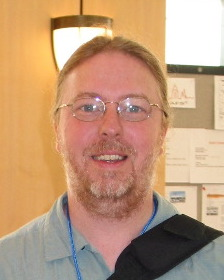
\includegraphics[width=\linewidth]{mugs/matt.jpg}

      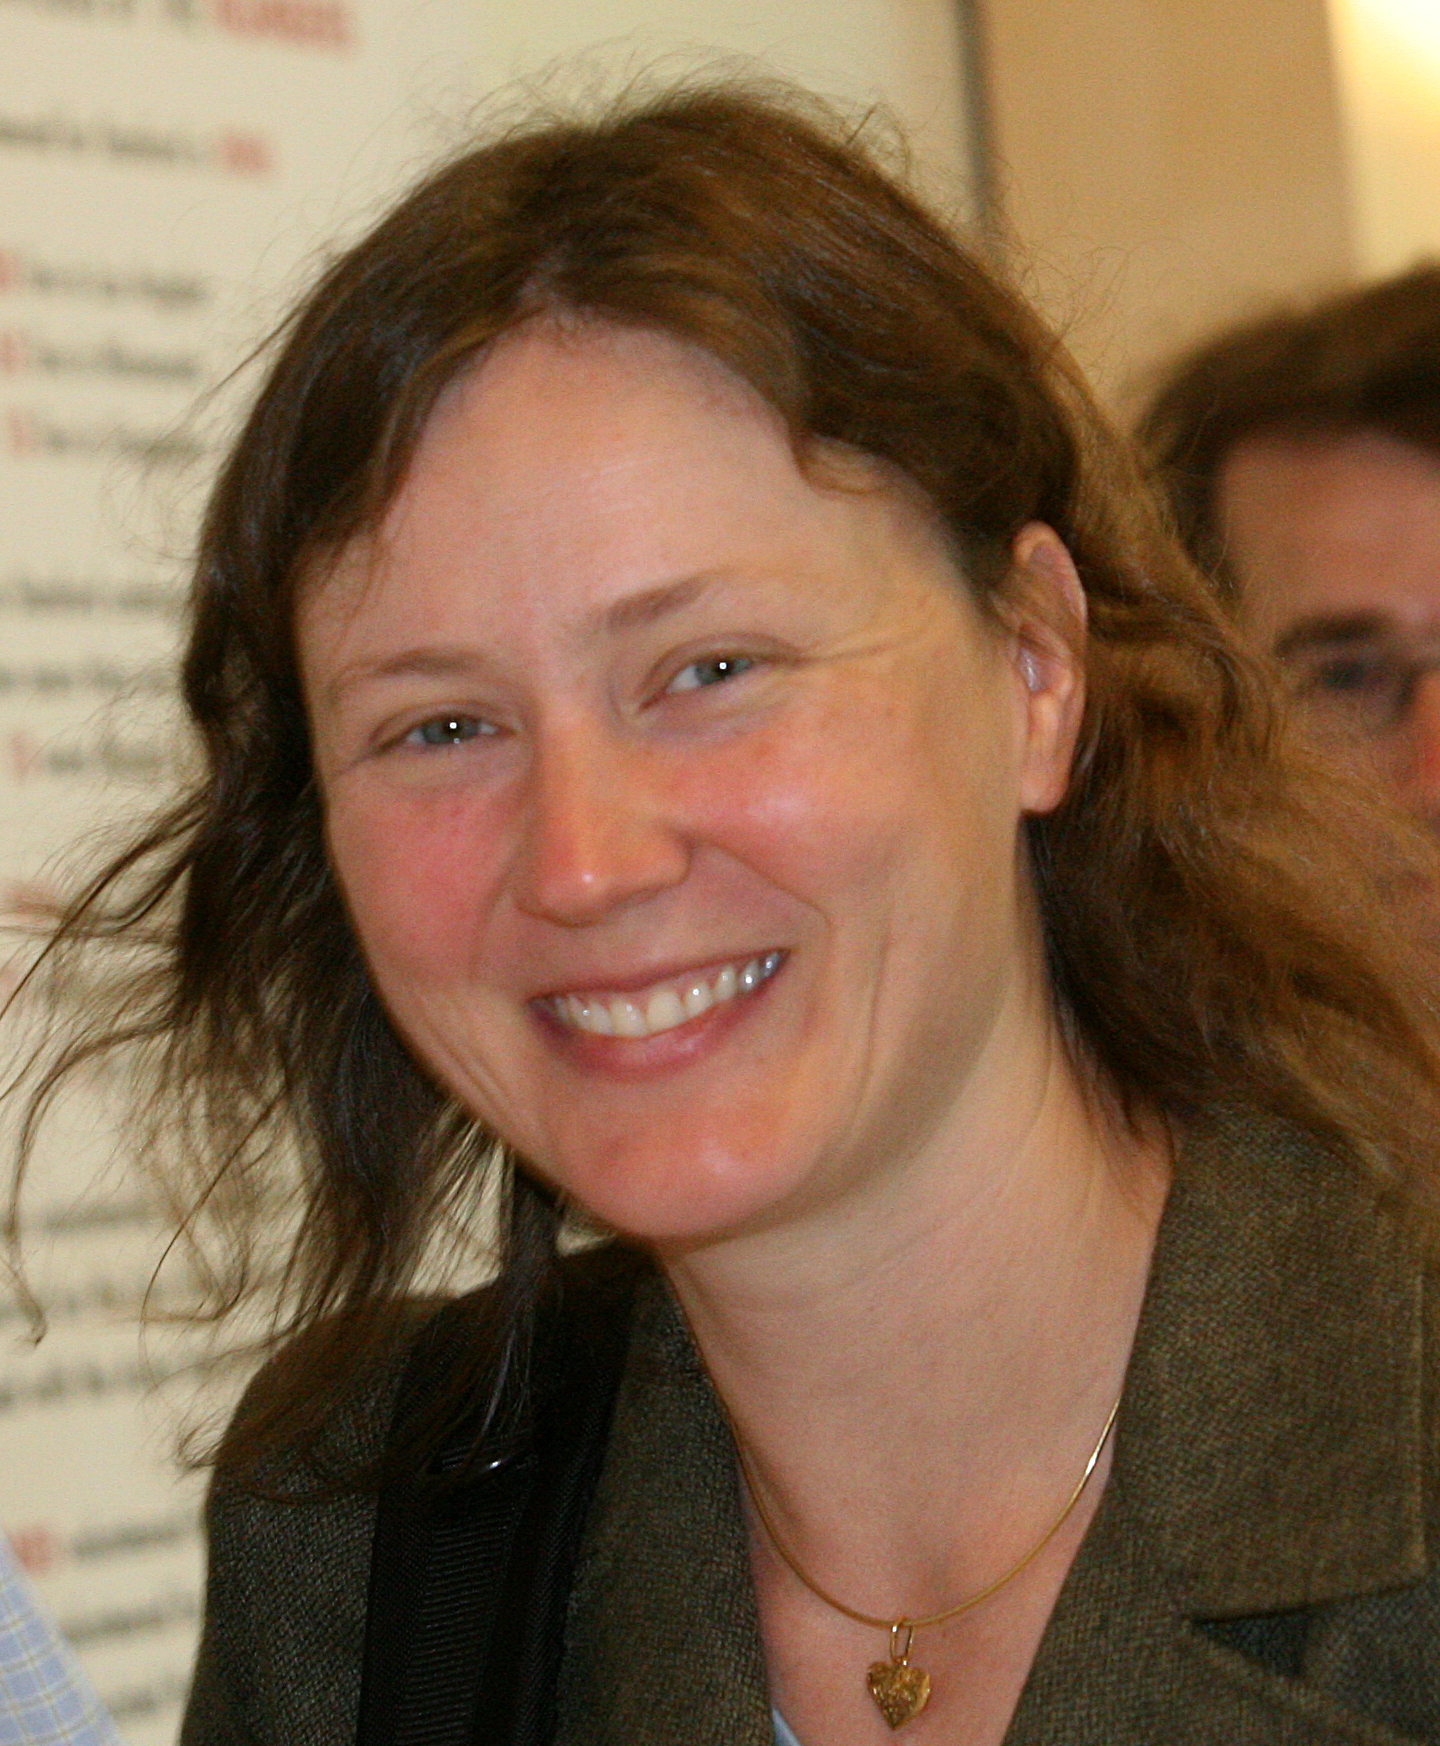
\includegraphics[width=\linewidth]{mugs/shelly.jpg}

      %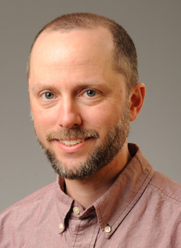
\includegraphics[width=\linewidth]{mugs/scott.jpg}
      
\includegraphics[width=\linewidth]{dummy.png}

      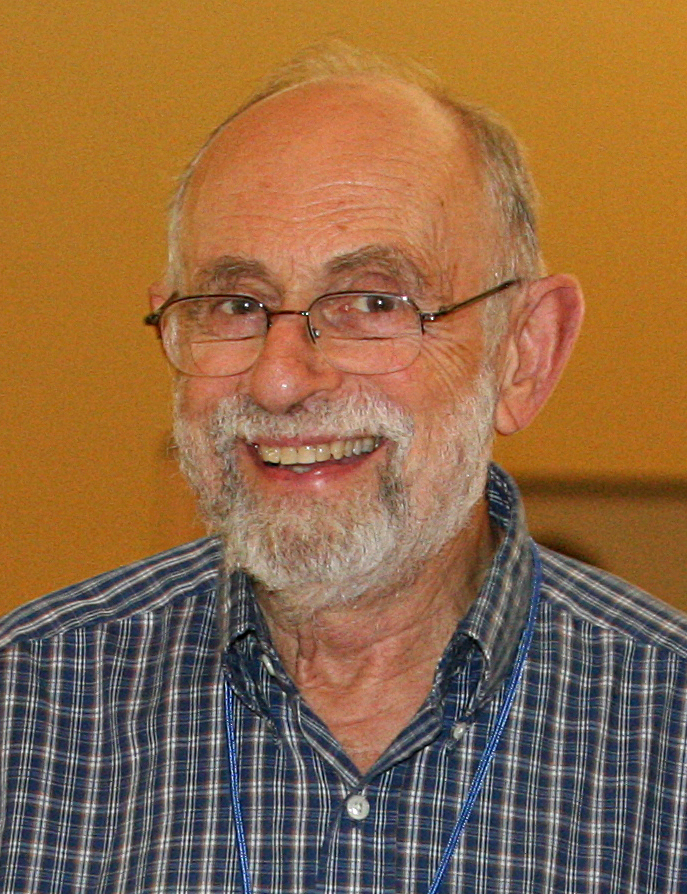
\includegraphics[width=\linewidth]{mugs/ed.jpg}

      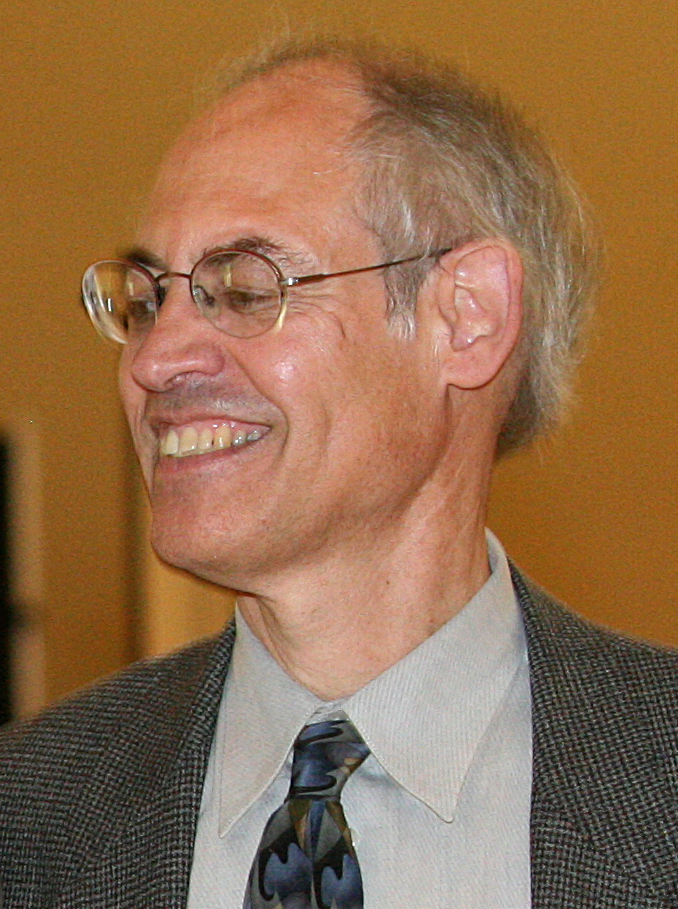
\includegraphics[width=\linewidth]{mugs/john.jpg}
    \end{column}
  \end{columns}
\end{frame}

\section{Why we measure XAS}

\begin{frame}
  \frametitle{The measurement goals of an XAS experiment}
  Picture of mu(E) beside a picture of a ball-n-stick structure

  Somehow the wiggles tell us something about the electronic 
  and atomic structure

  \begin{description}
  \item[Valence] the charge state of the absorber
  \item[Species] what kinds of atoms surround the absorber
  \item[Number] how many of those atoms there are
  \item[Distance] how far away they are
  \item[Disorder] how they are distributed due to thermal motion and
    structural disorder
  \end{description}
\end{frame}

\begin{frame}
  \frametitle{What can XAS be measured on}
  Well ... just about anything and on most element of the periodic table

  \begin{columns}[T]
    \begin{column}{0.5\linewidth}
      \begin{exampleblock}{No assumption of symmetry or periodicity}
        \begin{itemize}
        \item Crystals
        \item Liquids or amorphous/highly disordered solids
        \item Mixed phases
        \item Thin films and engineered materials
        \item Surface sorbed species
        \item Organic and organometallic species
        \item and on and on
        \end{itemize}
      \end{exampleblock}
    \end{column}
    \begin{column}{0.5\linewidth}
      \begin{alertblock}{Beamline choice and
          sample preparation matter}
        \begin{itemize}
        \item The beamline covers the absorber edge energy
        \item Sample is homogeneous
        \item Sample is not too thick, not too thin
        \item Sample is properly contained
        \end{itemize}
      \end{alertblock}
    \end{column}
  \end{columns}

\end{frame}

\begin{frame}
  \frametitle{Who uses XAS}
  Look to your left and right.  If you study catalysis, you may be
  sitting next to a biologist.  If you are a materials scientist, you
  might be sitting next to a geologist.

  \begin{block}{This fall, just at my beamline NSLS X23A2, my users include}
    \begin{itemize}
    \item 2 groups from the microelectronics industry
    \item 2 groups of electrochemists
    \item a group working on fuel cell catalysts
    \item a group working on photocathode materials
    \item a group working on nuclear waste containment
    \item a group working on materials for nuclear reactor vessels
    \end{itemize}
  \end{block}

  to say nothing of the biologists, enironmental scientists,
  geologists, and chemical scientists visiting the other beamlines at
  NSLS this fall.
\end{frame}

\section{How we measure XAS}

\begin{frame}
  \frametitle{Sometimes XAS is easy...}
  GeSb film
\end{frame}

\begin{frame}
  \frametitle{Sometimes XAS is hard...}
  Hg + DNA
\end{frame}

\begin{frame}
  \frametitle{Sometimes we do elaborate experiments}
  Spend several slides on
  \begin{itemize}
  \item imaging and $\mu$XAS
  \item qXAS and mountains of data
  \item DAFS
  \item NIXS
  \end{itemize}

\end{frame}

\section{How we use XAS}

\begin{frame}
  \frametitle{Fingerprinting}
  
\end{frame}

\begin{frame}
  \frametitle{XANES Interpretation}
  \begin{enumerate}
  \item Positioning
  \item Peak fitting
  \item Linear combination fitting
  \item Principle components analysis
  \end{enumerate}
\end{frame}

\begin{frame}
  \frametitle{XANES: Positioning}
  \begin{columns}
    \begin{column}{0.5\linewidth}
      Uranium 4+ and 6+ and intermediate
    \end{column}
    \begin{column}{0.5\linewidth}
      Farges
    \end{column}
  \end{columns}
\end{frame}

\begin{frame}
  \frametitle{XANES: Peak fiting}
  titanate perovskites?
\end{frame}

\begin{frame}
  \frametitle{XANES: Linear Combination Fitting}
  In this example, XAS is measured as a function of time as a gold
  chloride is reduced to metallic gold in the presence of sulfurous
  biomass.  At an intermediate time step, the spectrum is understood
  as a linear combination of the initial state
  ({\color{Green4}Au$^{3+}$Cl}), the final state ({\color{Purple4}Au
    metal}), and an intermediate state ({\color{Orange2}some Au$^{1+}$
    sulfide species}).
  \begin{columns}
    \begin{column}{0.5\linewidth}
      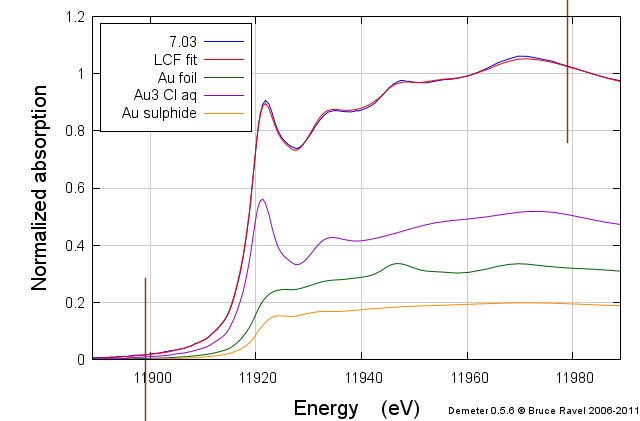
\includegraphics[width=\linewidth]{../iiss/xas/aucl_lcf.png}
    \end{column}
    \begin{column}{0.5\linewidth}
      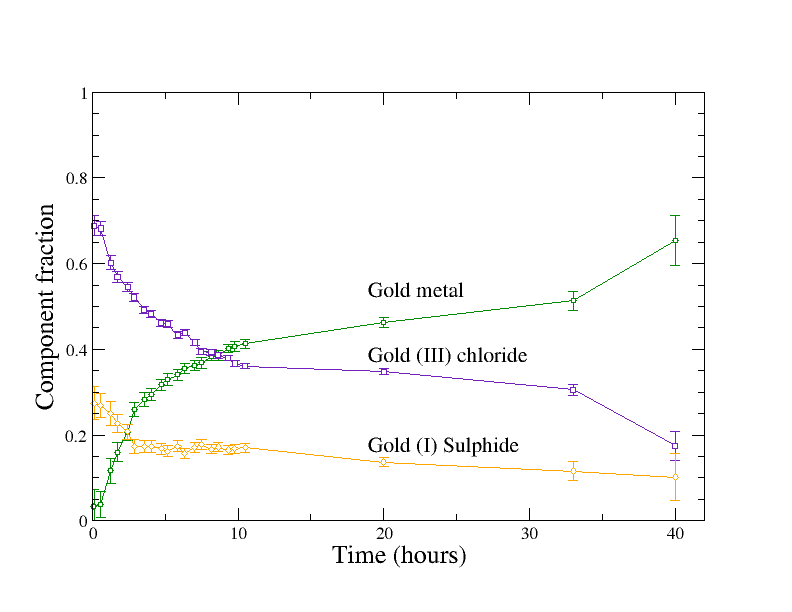
\includegraphics[width=\linewidth]{../iiss/xas/aucl_results.png}
    \end{column}
  \end{columns}
  \begin{flushright}
    \scriptsize (There will be an entire lecture on this topic tomorrow.)
  \end{flushright}
  \begin{textblock*}{0.5\linewidth}(0pt,18.75\TPVertModule) 
    \tiny
    M. Lengke et el., \textit{Mechanisms of Gold Bioaccumulation by
      Filamentous Cyanobacteria from Gold(III)-Chloride Complex},
    Environ. Sci. Technol. \textbf{40}(20) p.~6304-6309. (2006),
    \href{http://dx.doi.org/10.1021/es061040r}
    {\color{Blue4}\texttt{DOI: 10.1021/es061040r}}
  \end{textblock*}
\end{frame}

\begin{frame}
  \frametitle{XANES: Principle Components Analysis}
  Swipe something published
\end{frame}

\begin{frame}
  \frametitle{XANES: Theory}
  \begin{columns}
    \begin{column}{0.5\linewidth}
      Forward simulation
    \end{column}
    \begin{column}{0.5\linewidth}
      MXAN and FitIt
    \end{column}
  \end{columns}
\end{frame}

\begin{frame}
  \frametitle{EXAFS Analysis}
  
\end{frame}

\begin{frame}
  \frametitle{EXAFS analysis can be simple...}
  
\end{frame}

\begin{frame}
  \frametitle{EXAFS analysis can be sophisticated...}
  
\end{frame}

\begin{frame}
  \frametitle{EXAFS analysis can be quite elaborate...}
  Scott's mixed ferrites
\end{frame}

\section{How we understand XAS}

\begin{frame}
  \frametitle{Real space multiple scattering}
  
\end{frame}

\begin{frame}
  \frametitle{A bit of math}
  
\end{frame}

\begin{frame}
  \frametitle{The EXAFS equation}
  
\end{frame}

\begin{frame}
  \frametitle{XAS out of the vacuum}
  
\end{frame}

\begin{frame}
  \frametitle{XAS and statistics}
\end{frame}

\begin{frame}
  \frametitle{Ready, set, go!}
  \begin{alertblock}{}
    \begin{center}
      \LARGE \alert{Shall we begin?}
    \end{center}

  \end{alertblock}
\end{frame}
\end{document}
